\documentclass[letterpaper, 10pt, onecolumn, draftclsnofoot]{IEEEtran}
\usepackage{enumitem}
\usepackage{geometry}
\usepackage{tabularx}
\geometry{margin=.75in}
\usepackage{url}
\usepackage{graphicx}
\graphicspath{{./images/}}
\usepackage{float}
\usepackage{section}[placeins]
\usepackage{titlesec}
\titlelabel{\thetitle.\quad}
\usepackage{cite}
\usepackage{listings}

% Code Listing Settings
\lstset{language=[Sharp]C,
  showspaces=false,
  showtabs=false,
  breaklines=true,
  showstringspaces=false,
  breakatwhitespace=true,
  escapeinside={(*@}{@*)},
  commentstyle=\color{greencomments},
  keywordstyle=\color{bluekeywords},
  stringstyle=\color{redstrings},
  basicstyle=\ttfamily
}
\usepackage{color}
\usepackage{enumitem}

\definecolor{codegreen}{rgb}{0,0.6,0}
\definecolor{codegrey}{rgb}{0.5,0.5,0.5}
\definecolor{codeblue}{rgb}{0,0,0.6}
\definecolor{codered}{rgb}{0.6,0,0}
\definecolor{codeback}{rgb}{0.95,0.95,0.92}

\lstdefinestyle{mystyle}{
    backgroundcolor=\color{codeback},
    commentstyle=\color{codegreen},
    keywordstyle=\color{magenta},
    numberstyle=\tiny\color{codegrey},
    stringstyle=\color{codeblue}
}

\setlength\parindent{0pt}

% Section formatting settings
\renewcommand\thesection{\arabic{section}}
\renewcommand\thesubsection{\arabic{section}.\arabic{subsection}}
\renewcommand\thesubsubsection{\arabic{section}.\arabic{subsection}.\arabic{subsubsection}}

% TITLE / AUTHOR DATA
\title{\Large{\textbf{AR Sandbox for Construction Planning \\
                      Traffic Simulation Feature Update \\ 
                      \large{Winter Term Progress Update}}} \\
                      \vspace{15pt}}
                      
\author{Team Augmented Construction Education \\
       McKenzie~Gray,~Jonah~Spencer,~Adam~Sunderman}

% DOCUMENT BEGIN
\begin{document}

% TITLE
\maketitle
\vspace{100pt}

% Abstract
\begin{abstract}
    This document describes the progress our team has made over Fall and Winter terms on the AR Sandbox for Construction Planning. Overall project goals will be discussed first, followed by a demonstration and explanation in current beta level functionality of the new traffic simulation feature.    
\end{abstract}

% Table of Contents
\newpage
\tableofcontents
\clearpage
\newpage

% Section Project Purpose
\section{Purpose}
    The purpose of the AR Sandbox is mainly educational and meant as a means to visualize large-scale construction projects. The AR Sandbox offers a new and unique way for students to visualize the topics about which they learn in class with real-time feedback supported by various augmented reality modules.

% Goals
\section{Goals}
    The primary goal of this project is to introduce a traffic simulation mode, which includes AR marker functionality, to the AR Sandbox. The traffic simulation mode will project a visualization of a traffic simulation. Markers will be used to interact with the simulation in various ways, such as turning sections of road into work zones or introducing traffic lights to an intersection. After the scene has been modified by a marker, the traffic simulation will automatically update accordingly. \\
    
    Another important goal of this project is to improve the existing functionality of the AR Sandbox. Several aspects of the current AR Sandbox are not working properly, while other aspects need updates to make them more user-friendly. These improvements are described in the Problems section. \\
    
    Another feature to be added to the AR Sandbox is the ability to save and load scenes from any mode. For example, in depth mode, loading a previously-saved scene would project the heights from the saved scene onto the sand, thus indicating where sand must be placed in order to match the previous topography. In traffic simulation mode, loading a scene would result in the same road network as that of the saved scene.

% State of Development.
\section{Current State of Development}
    As the traffic simulation update is building on an existing project, the AR Sandbox is already fully-functional and supports three user modes: Depth Mode, Design Mode, and Cut \& Fill Mode. In Depth Mode, various colors are projected into the sandbox representing the current height of the sand. In Design Mode, a segment of road can be constructed by manipulating a variable number of control points.\cite{OrgOSUSandbox} Once the road segment has been created, it will be displayed using different colors representing whether sand needs to be added or removed in order for the road to be at the appropriate height. Finally, in Cut \& Fill Mode, a table collects and displays data from Design Mode that indicates the area and volume of cut and fill to be performed for the segment of road. \\
    
    The AR Sandbox currently uses a Microsoft Kinect V2 sensor for depth sensing and an Optoma ST50 projector for displaying the program window in the sandbox. The software is built on the Unity game engine, and the Kinect SDK is used to read depth data from the Kinect sensor. Additionally, a Logitech C920 webcam has been introduced to the AR Sandbox for use with Vuforia.
    
    \subsection{Winter Term Changes}
        The majority of the code involved in creating and loading a simulation network into Unity is complete but needs a few minor changes. Simulation road networks and terrains are building with no errors but still need to be properly textured, scaled, and aligned in the scene.\\
        
        Vuforia interactions are ready for use in some places but need to be integrated with the rest of the system. The current user interface will be changed to use Vuforia's Virtual Buttons and marker interaction will be introduced once simulations are fully-functional.\\
        
        The simulation logic and visuals that will run on networks and terrains is one of the more challenging tasks and requires that network creation be stable before implementation. This feature is in progress but cannot yet be demonstrated for this document.\\
        
        The original AR Sandbox depth mode has been upgraded. The feature is now able to display contour lines on the elevation projection. As the projection changes color gradients, and therefore height, a black line is drawn between the change. This helps a user more precisely determine height information in places where there are greater rates of change in elevation. \\

% What is still needed.
\section{Outstanding Task List}
    \subsection{Network Creation and Loading}
        \begin{enumerate}
            \item Adjust textures and materials for models.
            \item Ensure all models are properly scaled, rotated, and translated.
            \item Finish the building model procedural algorithm to add buildings to a simulation.
            \item Add scene objects with interaction. Traffic lights, stop signs, etc.
            \item Add scene objects with no interactions. Benches, trash cans, street lights, etc.
        \end{enumerate}
        
    \subsection{Vuforia Integration}
        \begin{enumerate}
            \item Connect user interface to Vuforia using Virtual Buttons.
            \item Apply marker interaction to traffic simulation scene objects.
        \end{enumerate}
    
    \subsection{Simulation Visuals and Logic}
        \begin{enumerate}
            \item Create a client-server based class for interacting with Traci to get simulation data.
            \item Create models for different vehicle representations.
            \item Define the specific macroscopic logic for simulation color coding.
            \item Create a user interface to switch between the macroscopic and microscopic simulation modes.
            \item Develop algorithm to determine passing lanes for simulation vehicles. (Line-Of-Sight)
        \end{enumerate}
        
    \subsection{Upgrades to Existing AR Sandbox}
        \begin{enumerate}
            \item Saving and loading of terrains.
            \item Depth mode calibration improvement.
            \item Fix exception errors in the old 'design' mode.
        \end{enumerate}
        
% Problems
\section{Problems}
    \begin{enumerate}[label=]
        \item{\textbf{Remounting the projector and depth camera:}}
            In order to create a more permanent and appealing mount for the projector and camera we researched a few mounting options. For the Kinect depth camera we will just drill a couple holes in the plastic frame and attach it with screws to the AR Sandbox. Mounts are available, but not necessary. The projector mount needed to be low-profile and have adjustments for rotation and pitch. After looking at GoPro action camera mounts and projector mounts we ended up using a mount designed for trail cameras used to photograph wildlife.
        
        \item{\textbf{Replacing the sand in the AR Sandbox:}}
            The sand in the AR Sandbox was determined to be too glassy by the client and he wished to find a more suitable sand that didn't reflect light as well. Research found that most sands other than play sand (which the AR Sandbox has) contain carcinogens. We have decided that it is better to deal with the reflection from the projector rather than risk of harm to the users of the AR Sandbox.
            
        \item{\textbf{Cleaning up previous work on the AR Sandbox:}}
            Several aspects of the current AR Sandbox are not working properly, while other aspects need updates to make them more user-friendly. Some known needed improvements include:
            \begin{itemize}
                \item{} 
                    The settings for minimum and maximum height in calibration mode are very sensitive and it can be very difficult to get them to the right setting.
                \item{} 
                    Switching modes via the menu does not always work, and keyboard shortcuts must be used instead.
                \item{} 
                    In Design Mode, adding a control point throws an exception and causes one of the endpoints to stop functioning properly. There are likely many small bugs like this one that we will need to fix
            \end{itemize}
        
        \item{\textbf{Making the AR Sandbox usable during development:}} 
            To make the AR Sandbox usable by students and professors during development of new features we will build a version of the app in its current state. This version will be named ARSandbox2018-Stable and will be available as source code on GitHub in it's current state as well.
        
        \item{\textbf{Using Vuforia with the Kinect camera:}} 
            For the first several weeks of development, Vuforia was unable to track images consistently. We determined early on that the Kinect was somehow distorting the image, making it next to impossible for Vuforia's computer vision to recognize images. After modifying settings within Unity, Vuforia, and the Kinect API, we were unable to resolve the problem. Instead, we installed a new webcam on the AR Sandbox for use solely with Vuforia.
    \end{enumerate}

% Beta Functionality Demonstration
\section{Beta Functionality Demonstration}
    The following images and captions give a detailed example of creating a traffic simulation network with the AR Sandbox. First, a real world location will be selected to be used as the simulation model and it's data will be downloaded from Open Street Map. Next, the locations roads, buildings, and a terrain will be built as Unity GameObjects and loaded into the game engine where simulations will be run with Vuforia interaction.

\newpage
\begin{figure}[h!]
    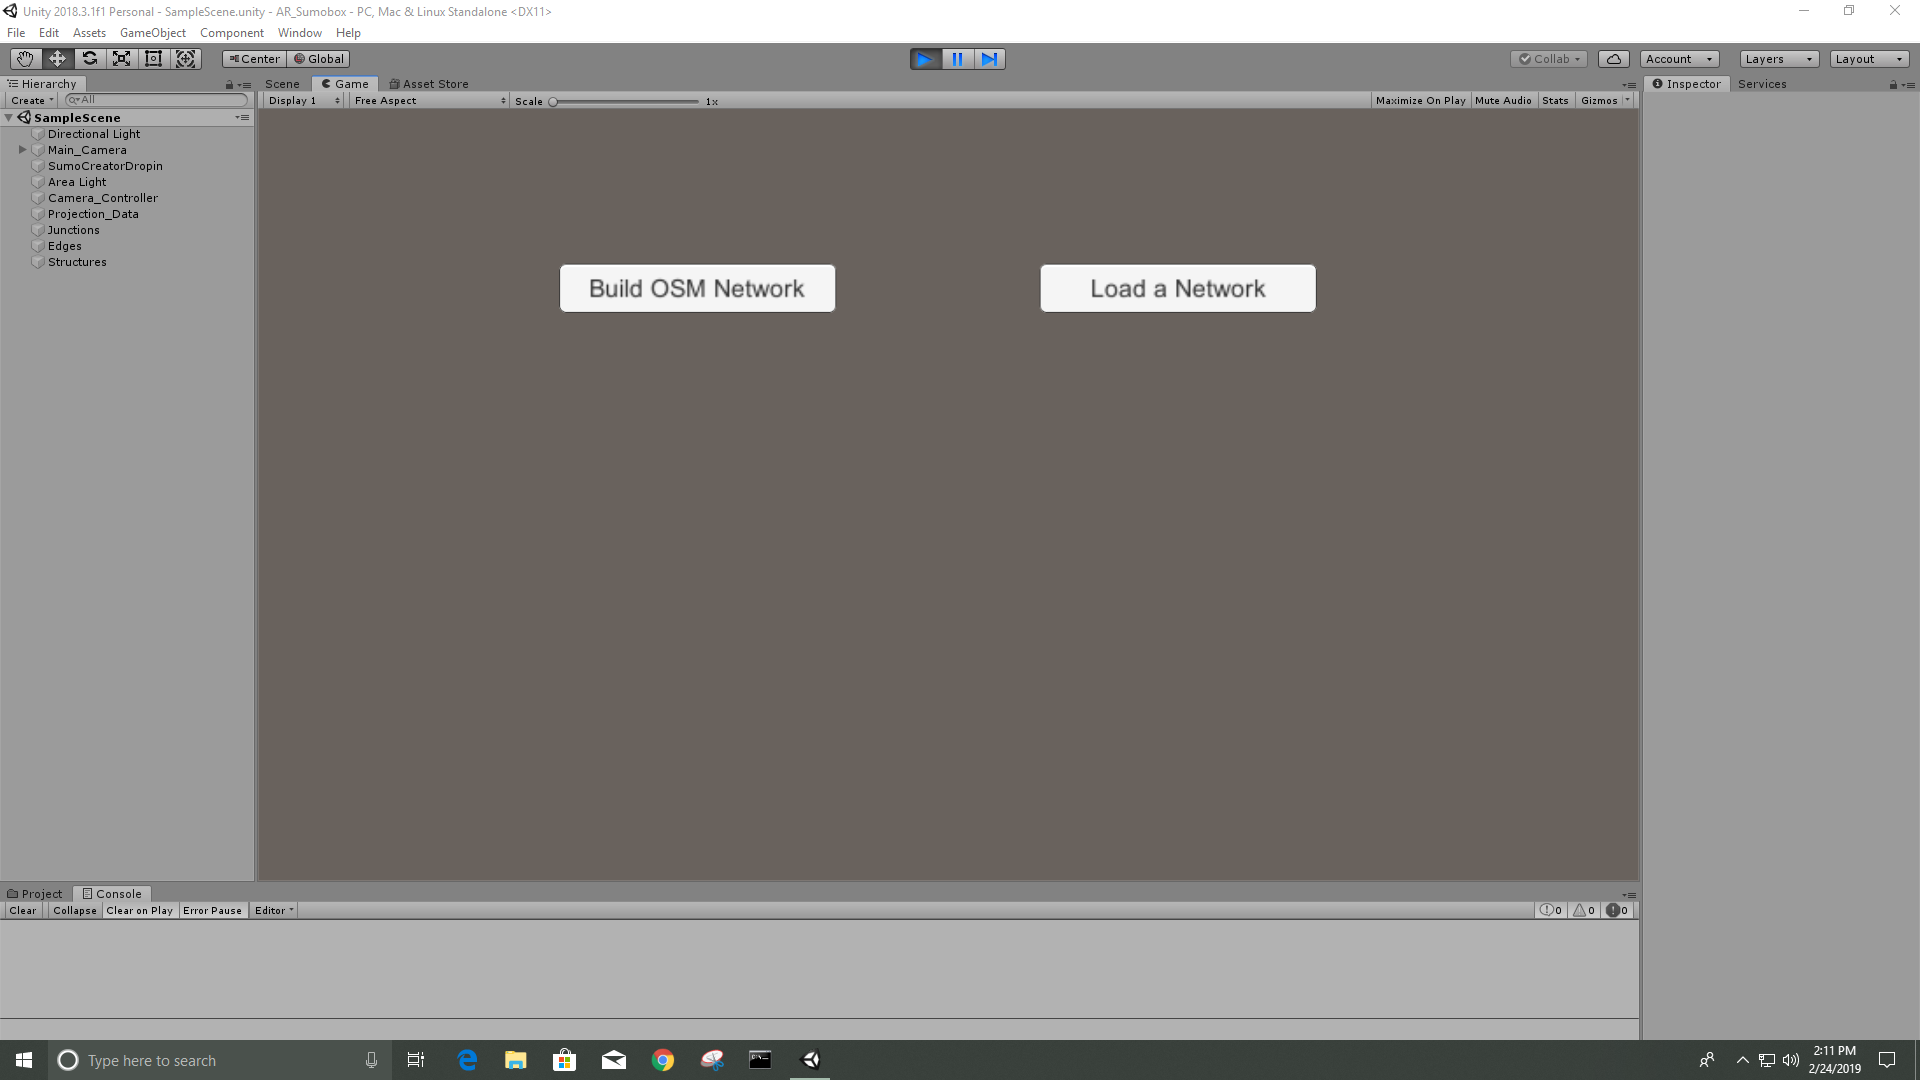
\includegraphics[width=\textwidth]{TempMenuScreen_1}
    \caption{The temporary menu screen for development and selecting the option "Build OSM Network".}
    \label{fig:my_label}
\end{figure}
\begin{figure}[h!]
    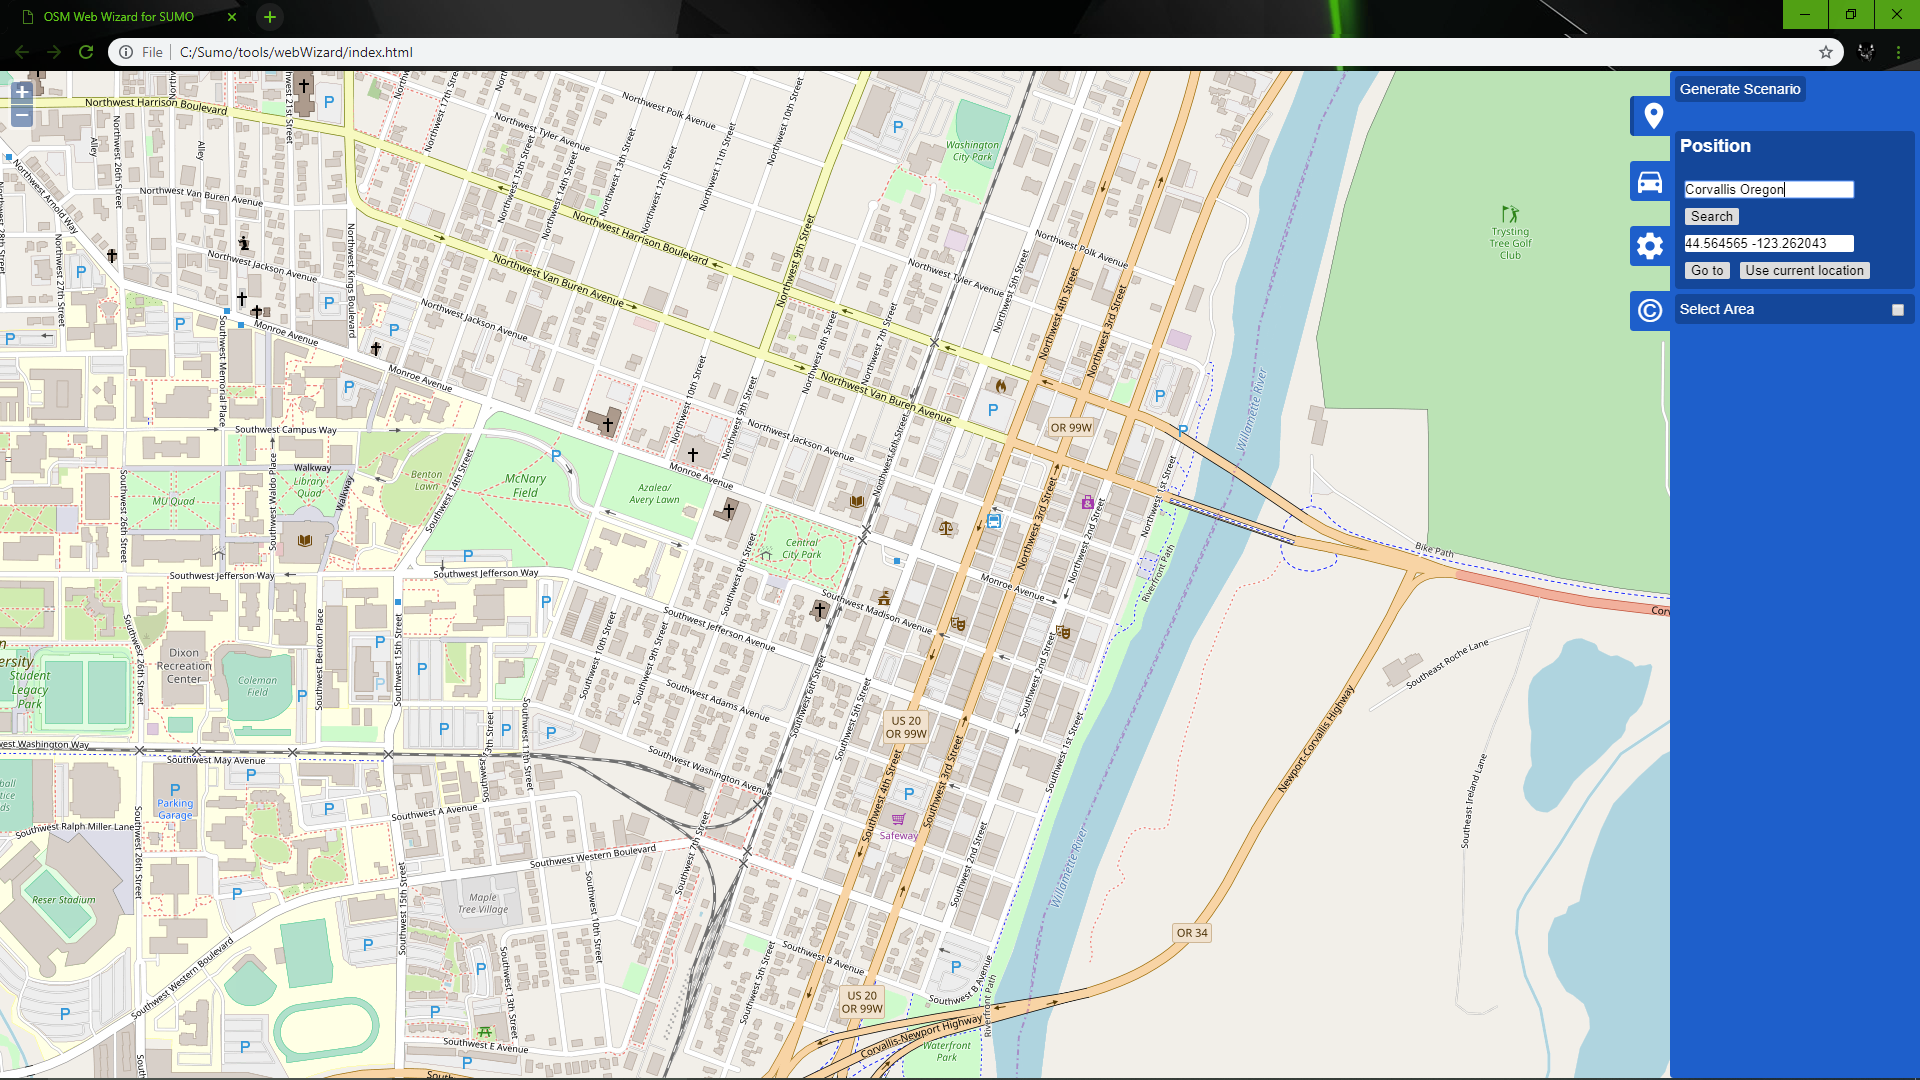
\includegraphics[width=\textwidth]{OsmCorvallisSelection_3}
    \caption{The import screen after typing "Corvallis Oregon" in the Position text box}
    \label{fig:my_label}
\end{figure}

\newpage
\begin{figure}[h!]
    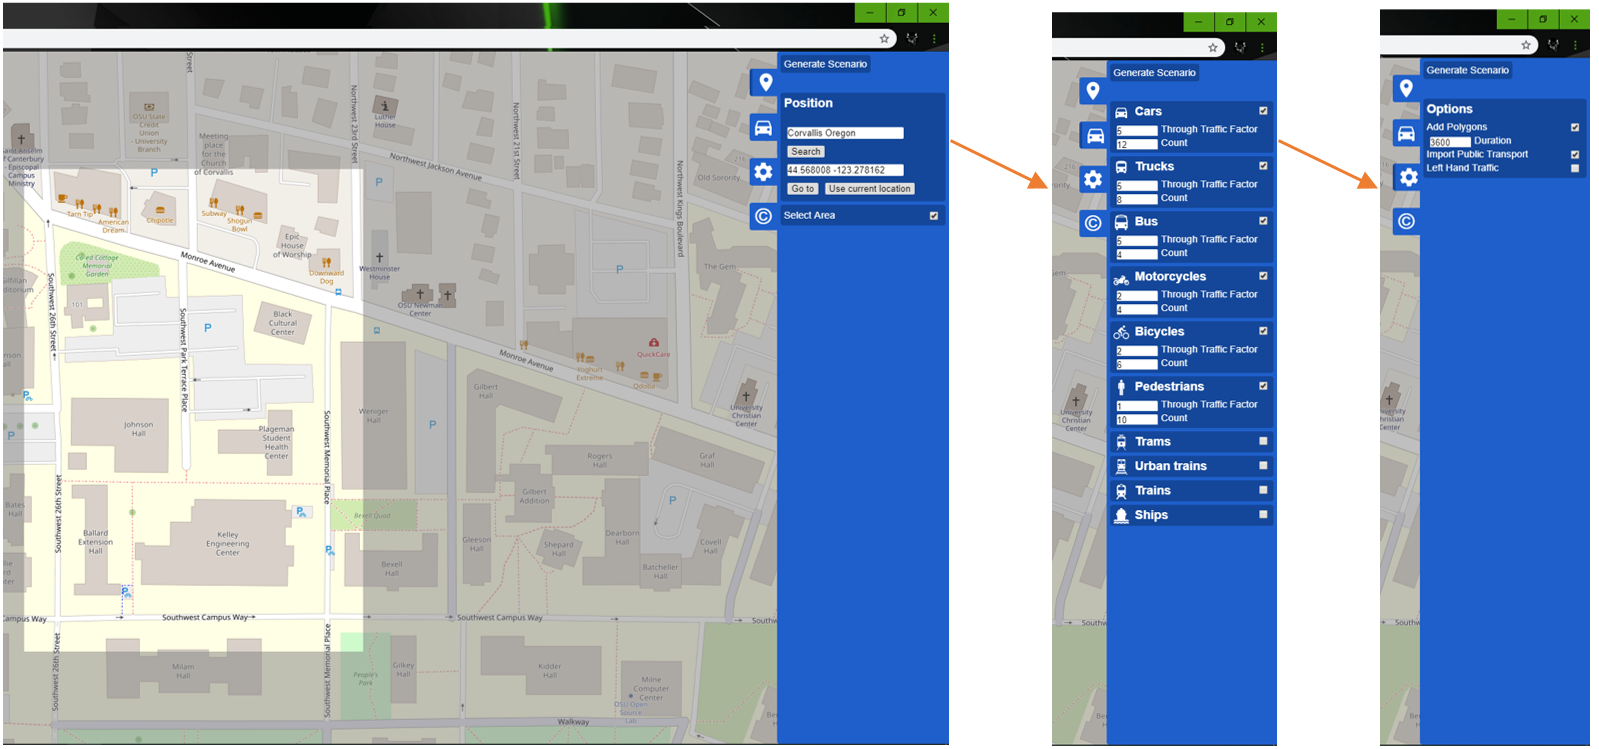
\includegraphics[width=\textwidth]{OSM_Settings}
    \caption{Map data is converting from Open Street Map format to SUMO required format.}
    \label{fig:my_label}
\end{figure}

\vspace{3pt}
\begin{figure}[h!]
    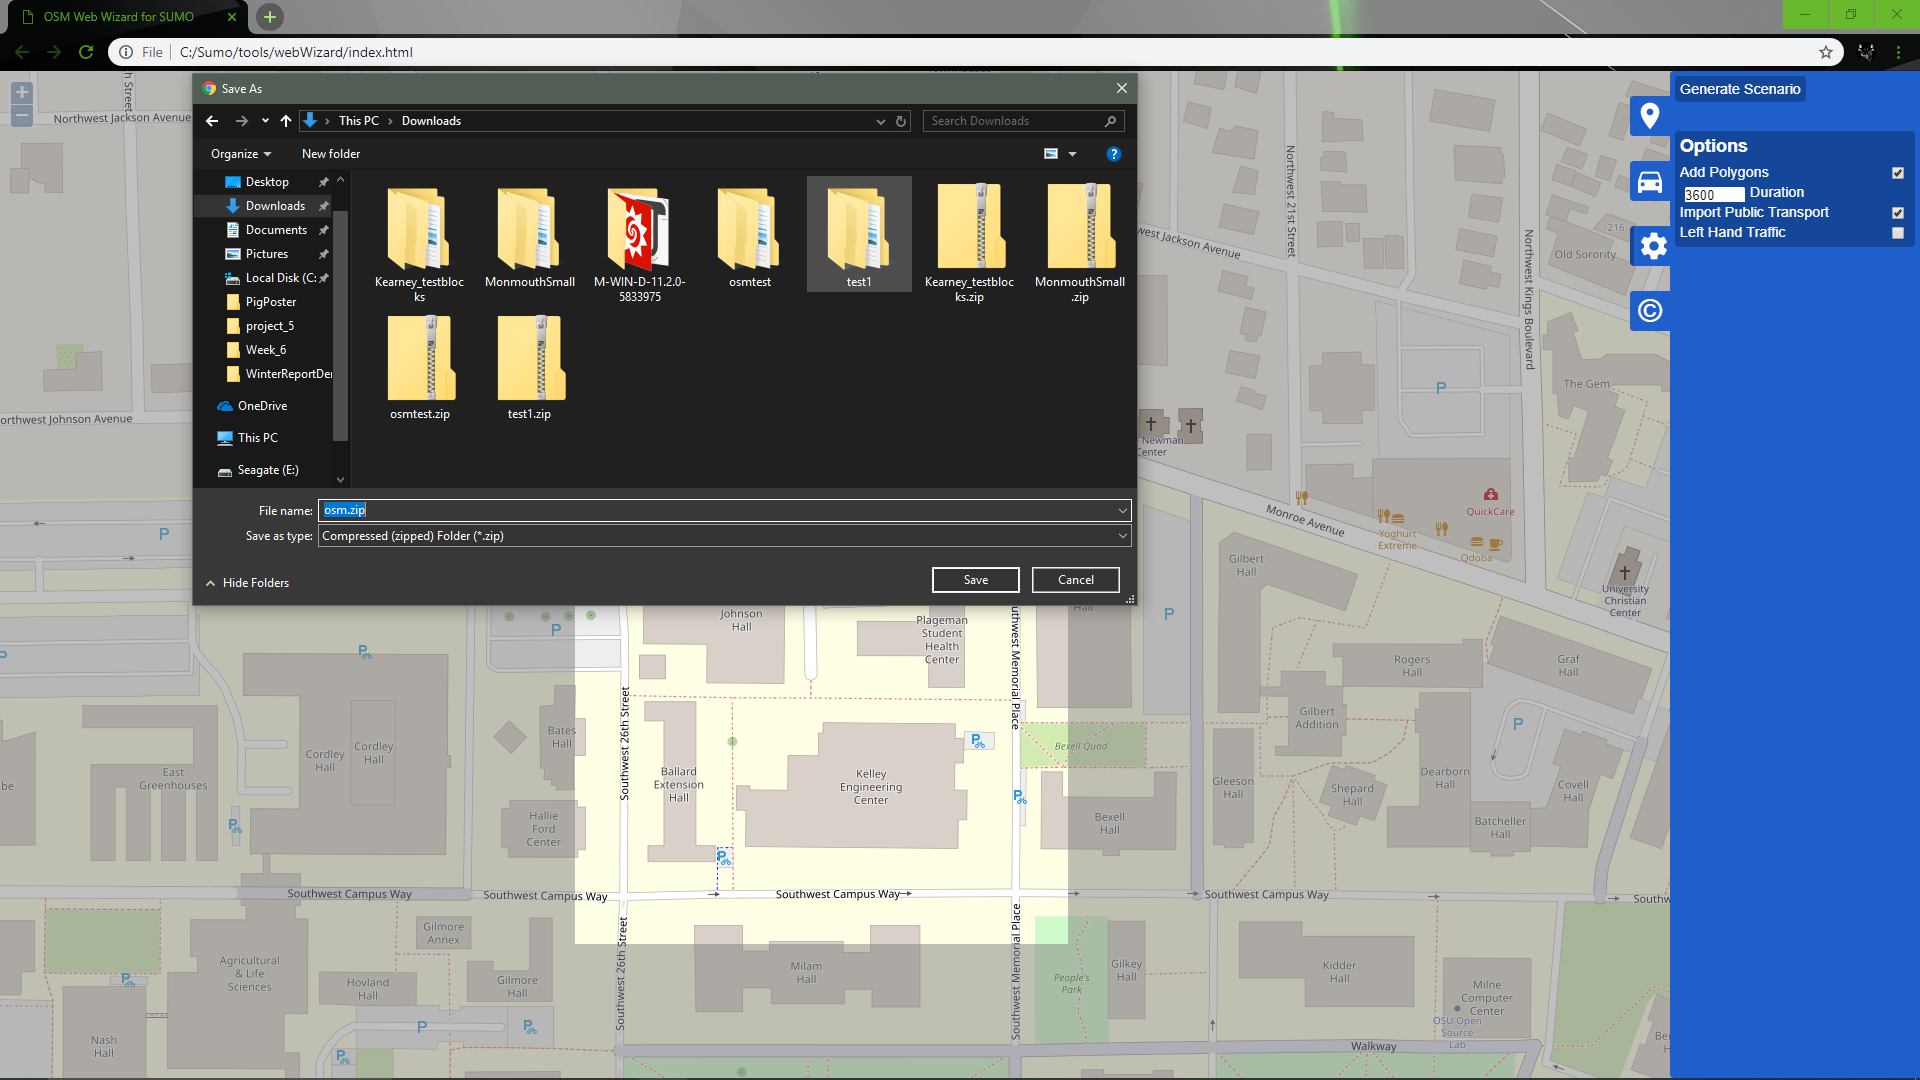
\includegraphics[width=\textwidth]{OsmDownloadZip_8}
    \caption{A dialog is opened which allows the user to save the new network as a zip file.}
    \label{fig:my_label}
\end{figure}
    
\vspace{3pt}
\begin{figure}[h!]
    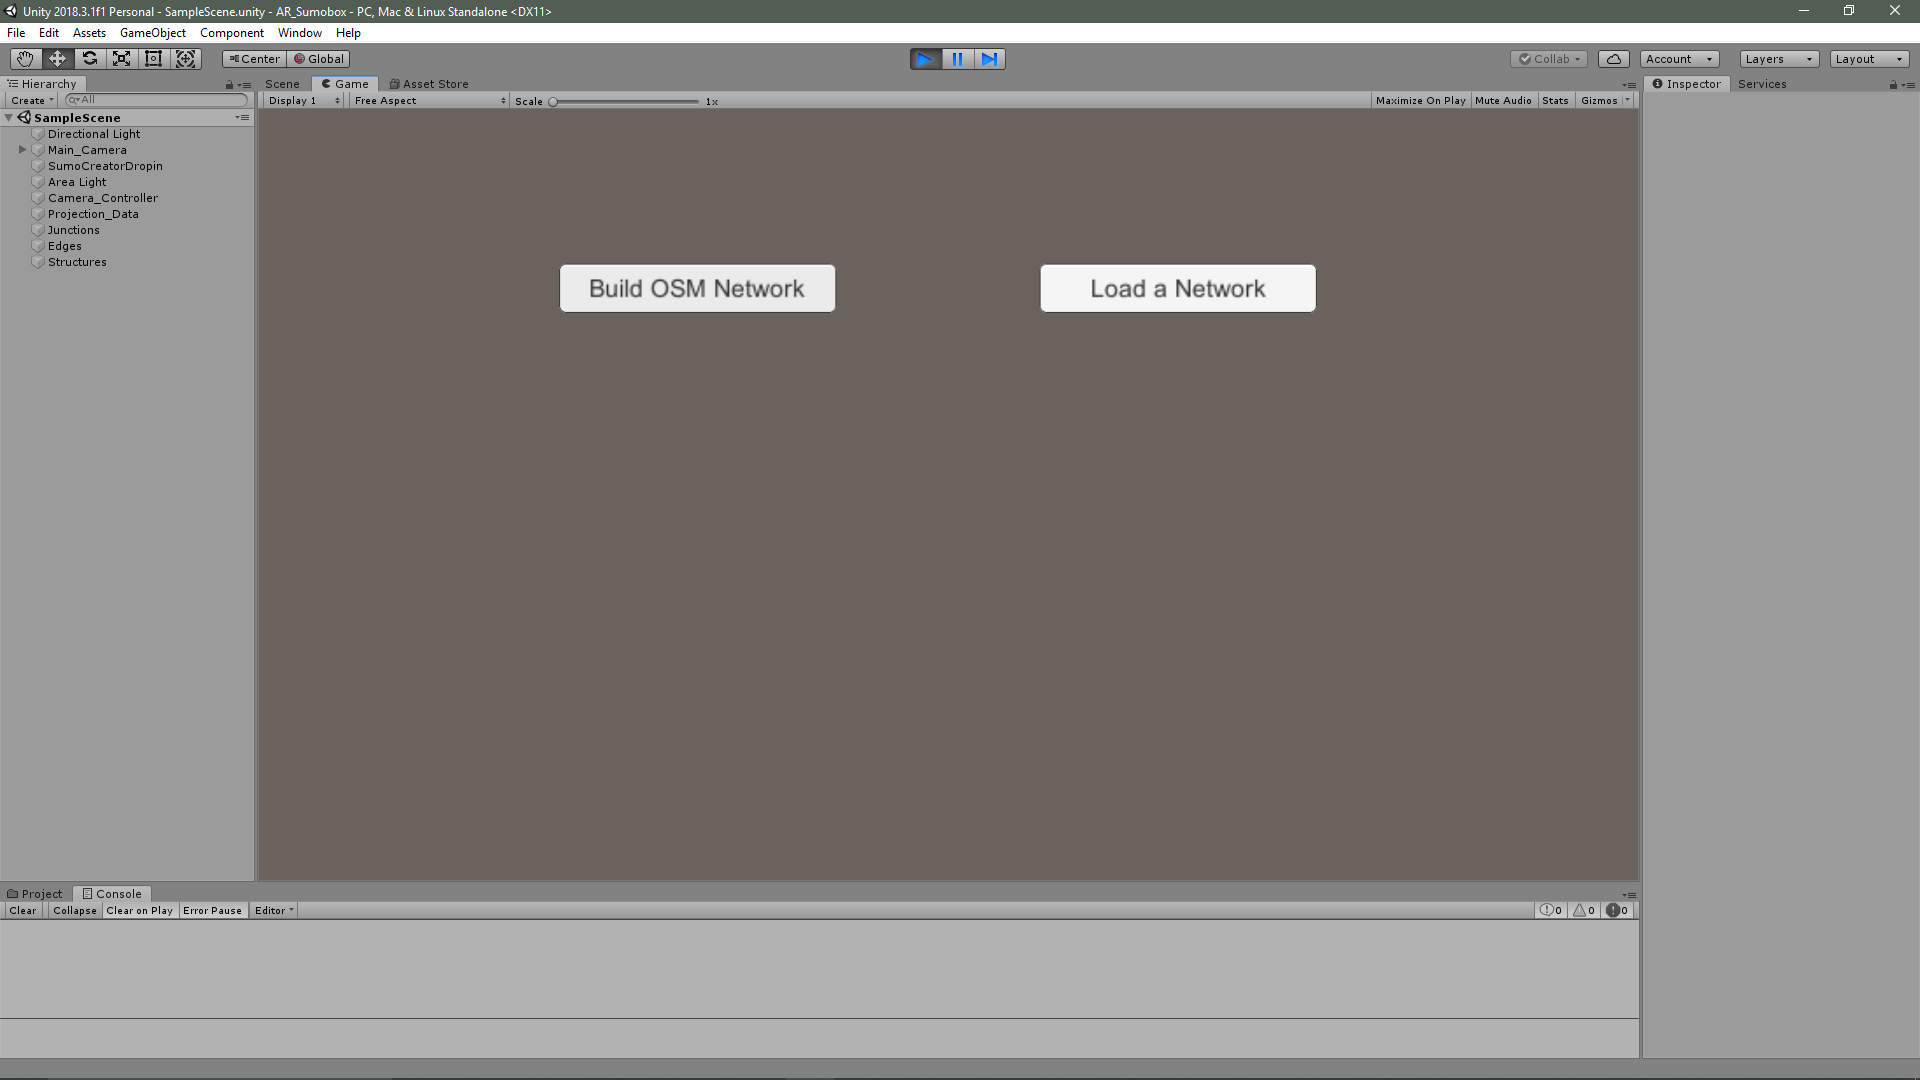
\includegraphics[width=\textwidth]{BackToUnityOsm_9}
    \caption{Back to the main menu and select the option "Load a Network".}
    \label{fig:my_label}
\end{figure}
\vspace{3pt}
\begin{figure}[h!]
    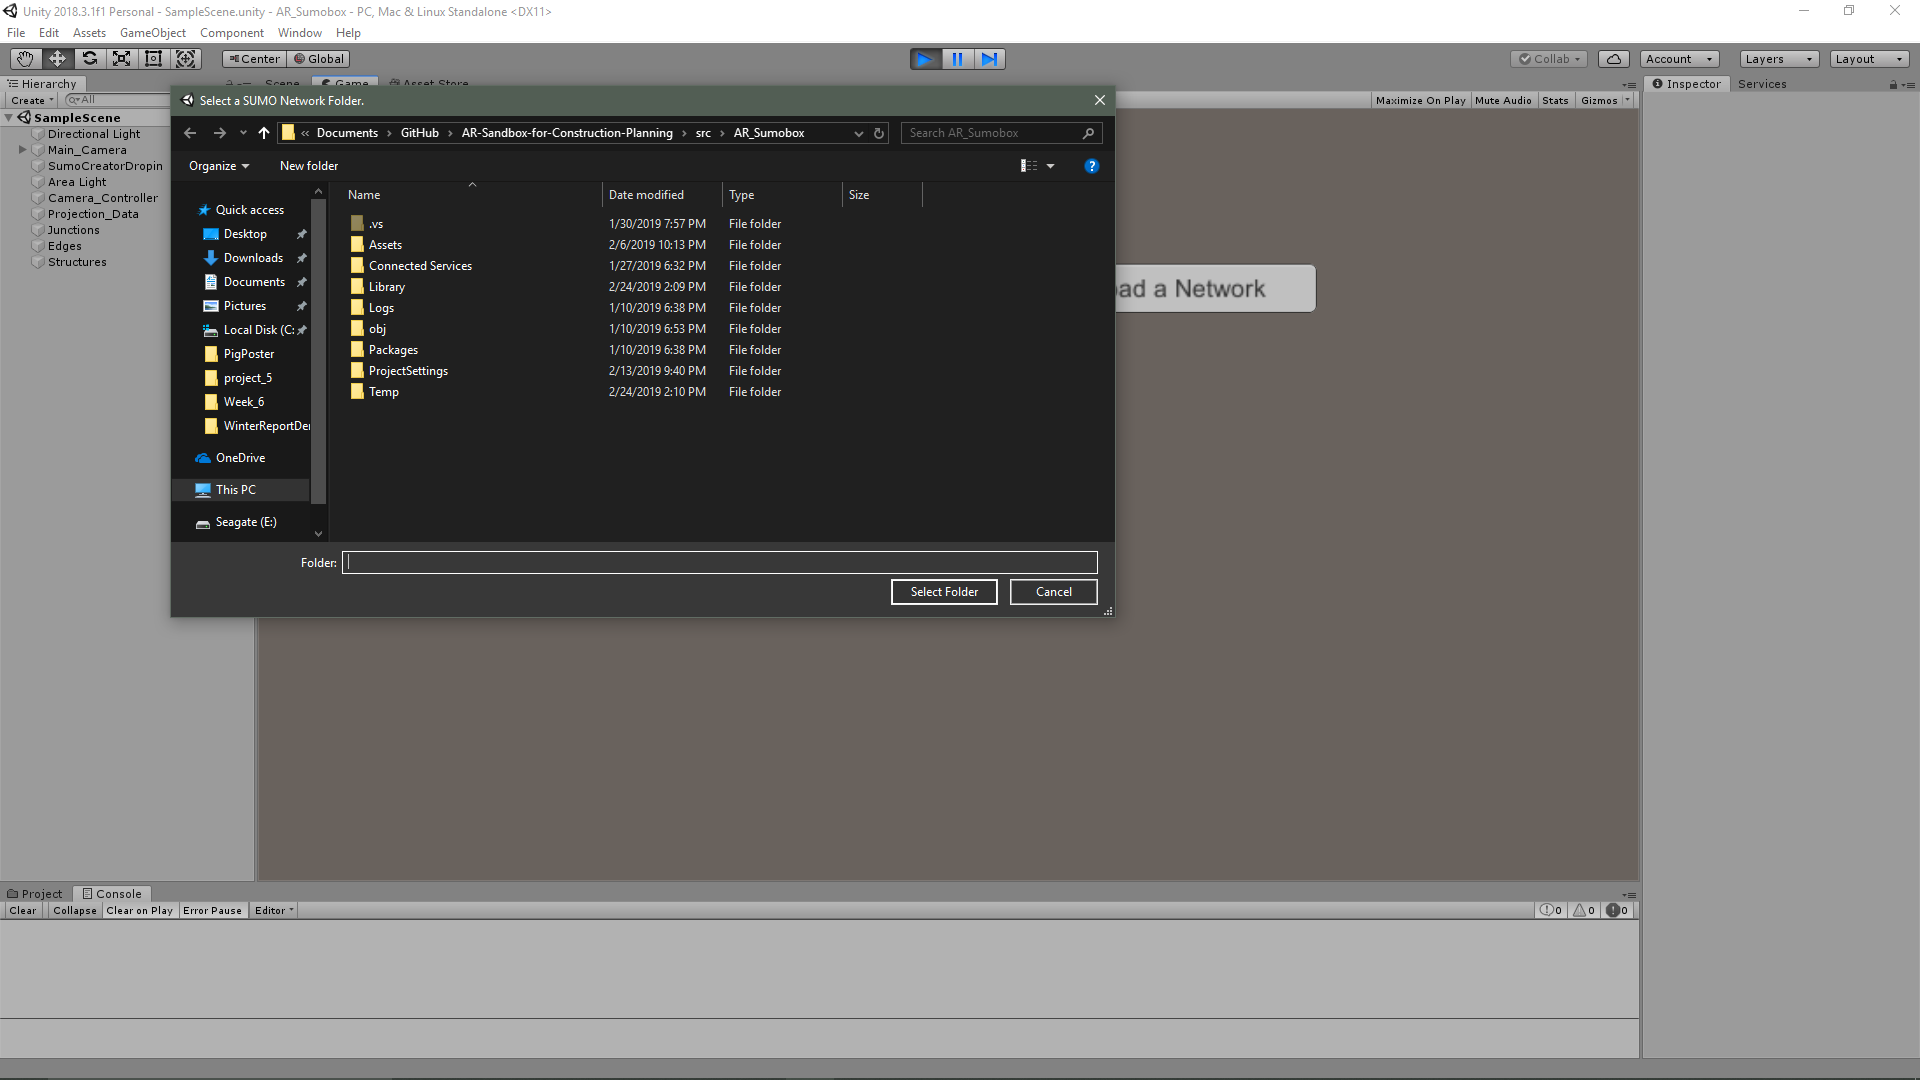
\includegraphics[width=\textwidth]{LoadNetworkSelected_10}
    \caption{A dialog is again opened so the user can choose a network to load into Unity.}
    \label{fig:my_label}
\end{figure}
\vspace{3pt}
\begin{figure}[h!]
    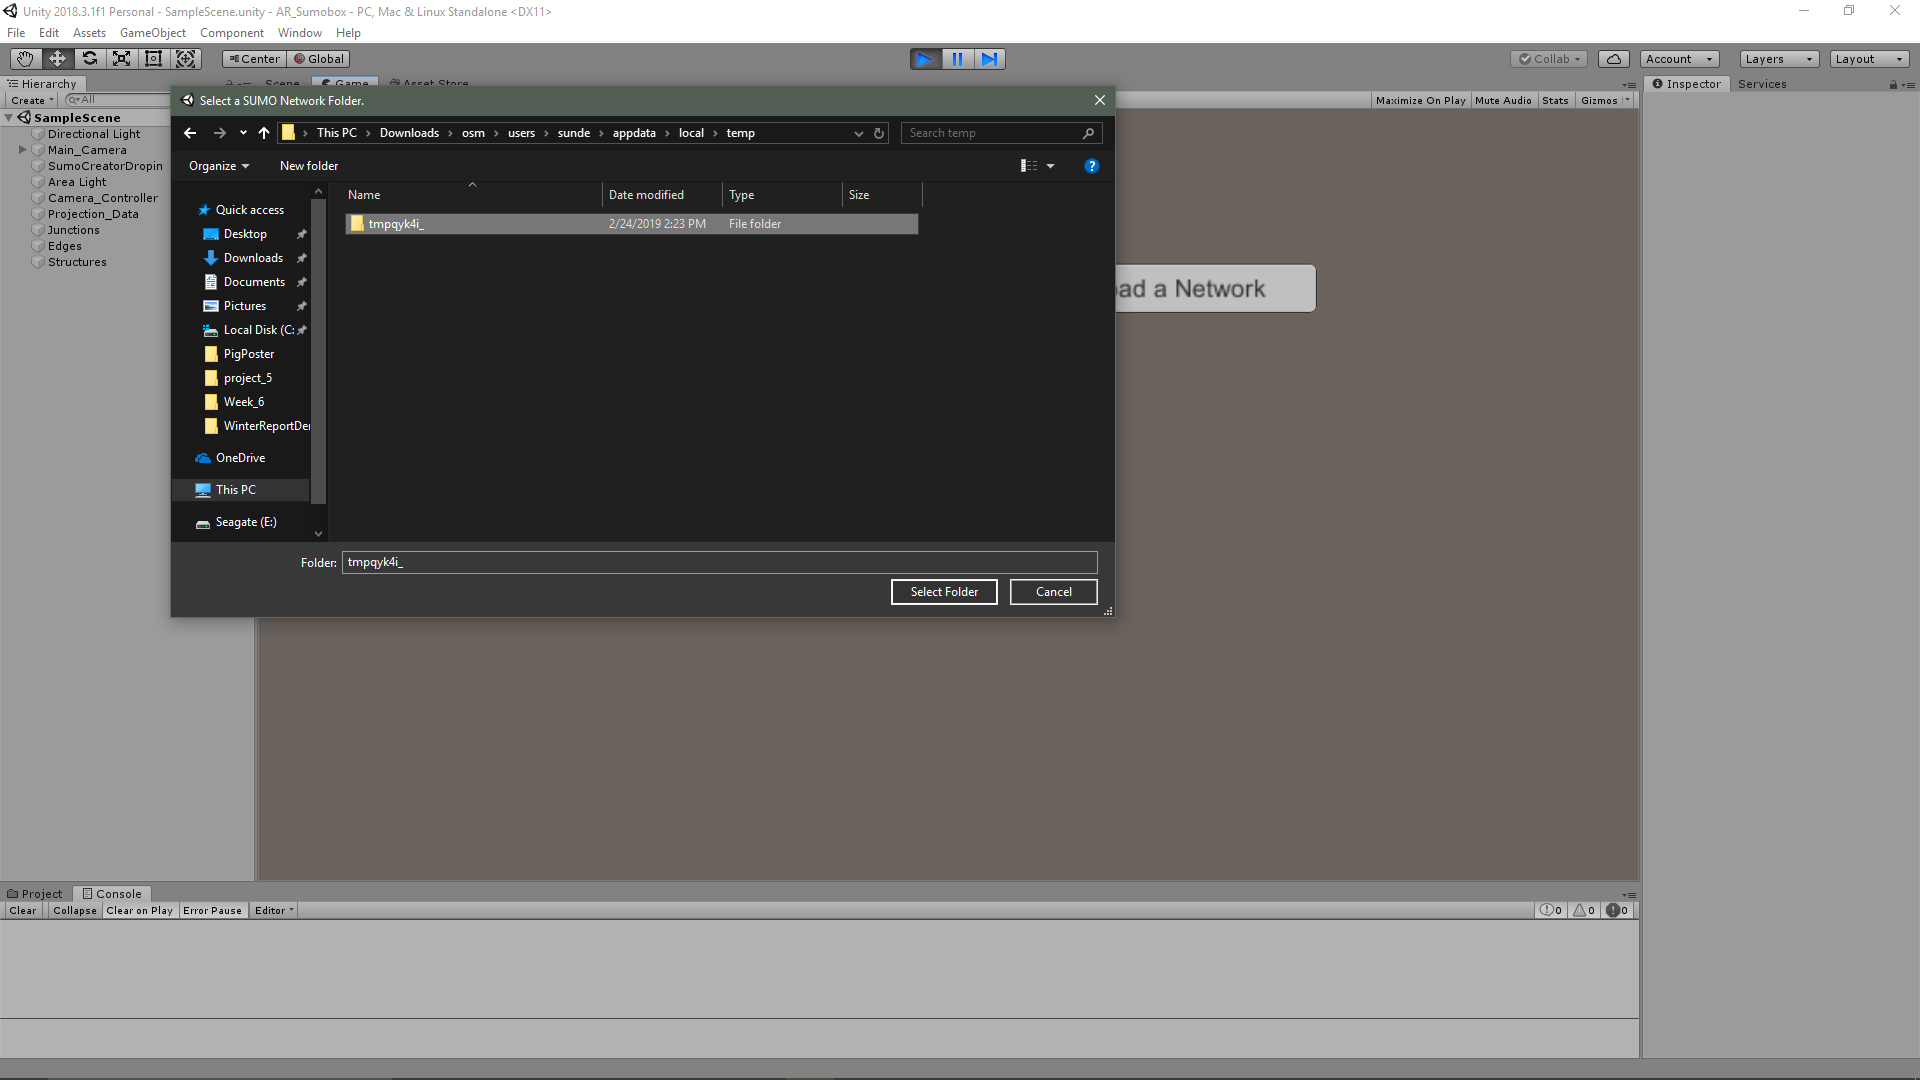
\includegraphics[width=\textwidth]{SelectFolder_11}
    \caption{We navigate to our networks root folder and choose "Select Folder".}
    \label{fig:my_label}
\end{figure}
\vspace{3pt}
\begin{figure}[h!]
    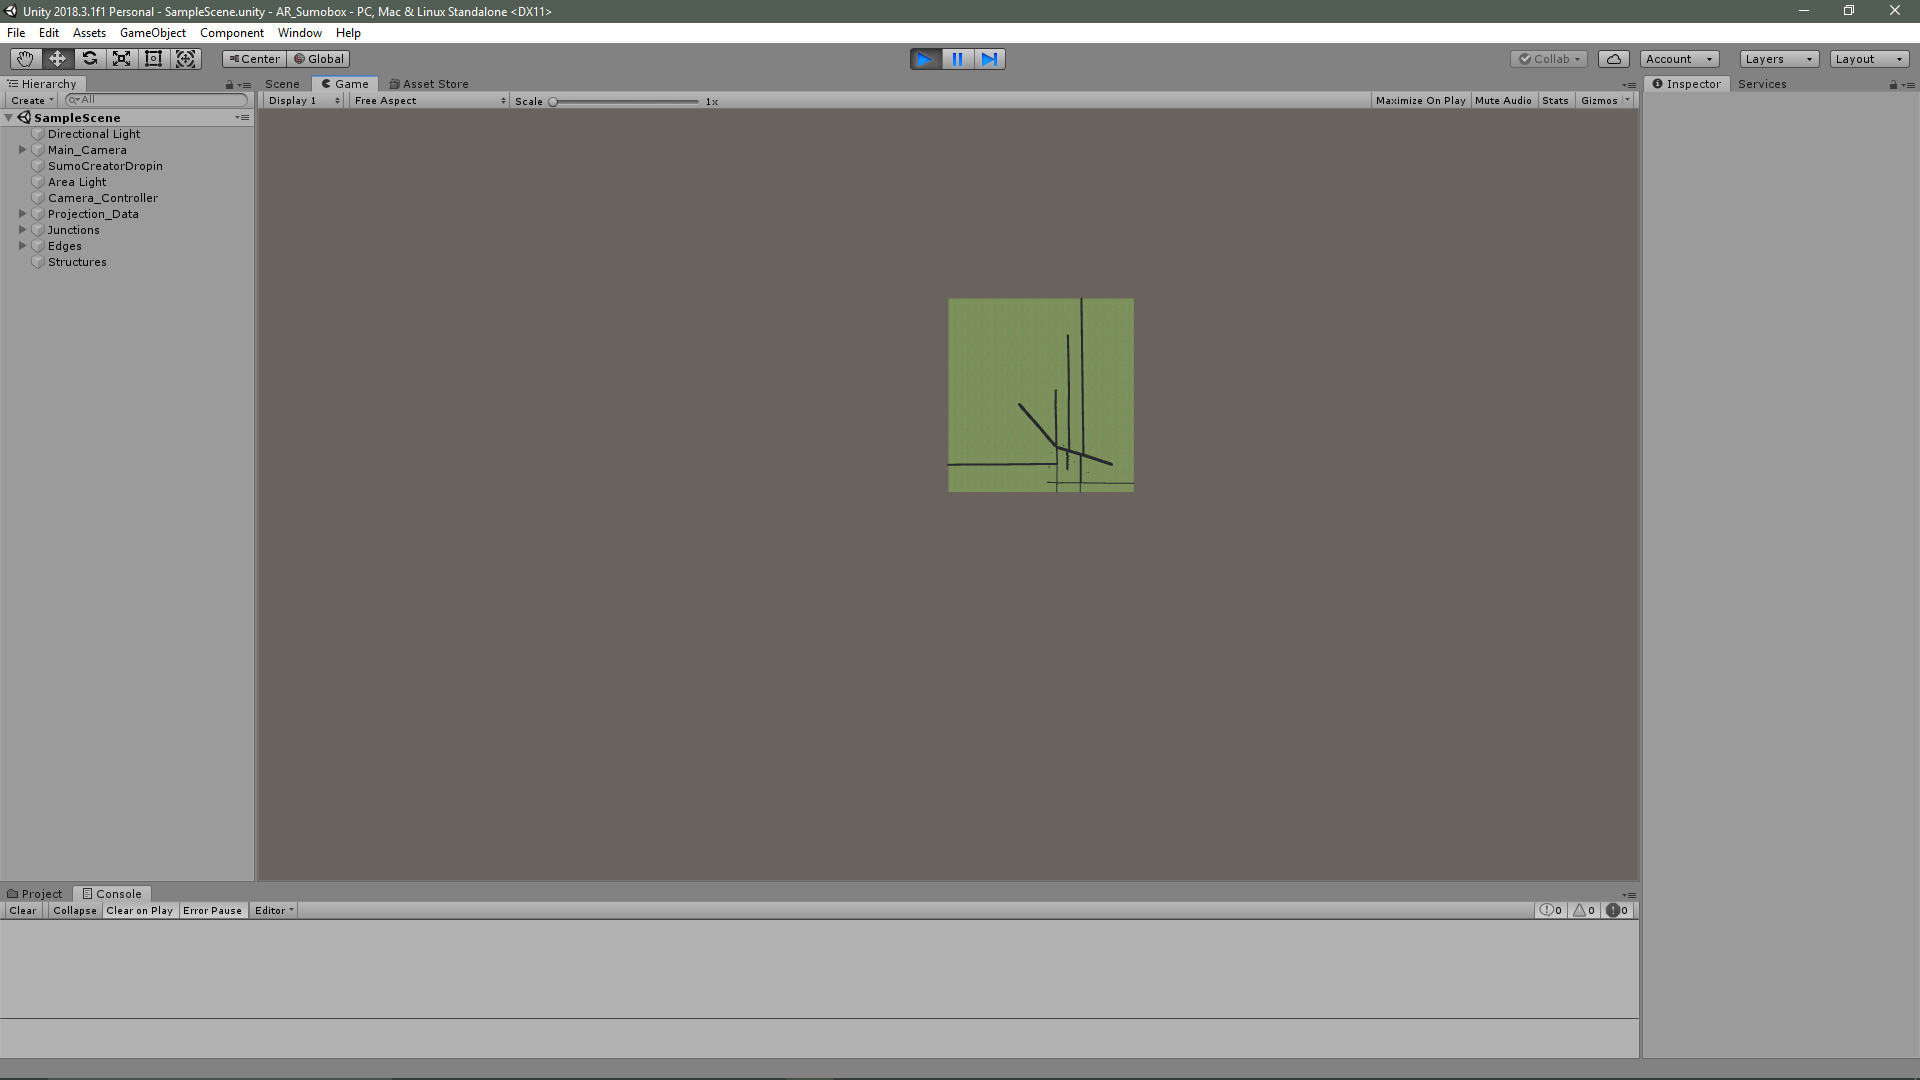
\includegraphics[width=\textwidth]{ViewAfterBuild_12}
    \caption{The network is loaded and we are presented a topdown view.}
    \label{fig:my_label}
\end{figure}
\vspace{3pt}
\begin{figure}[h!]
    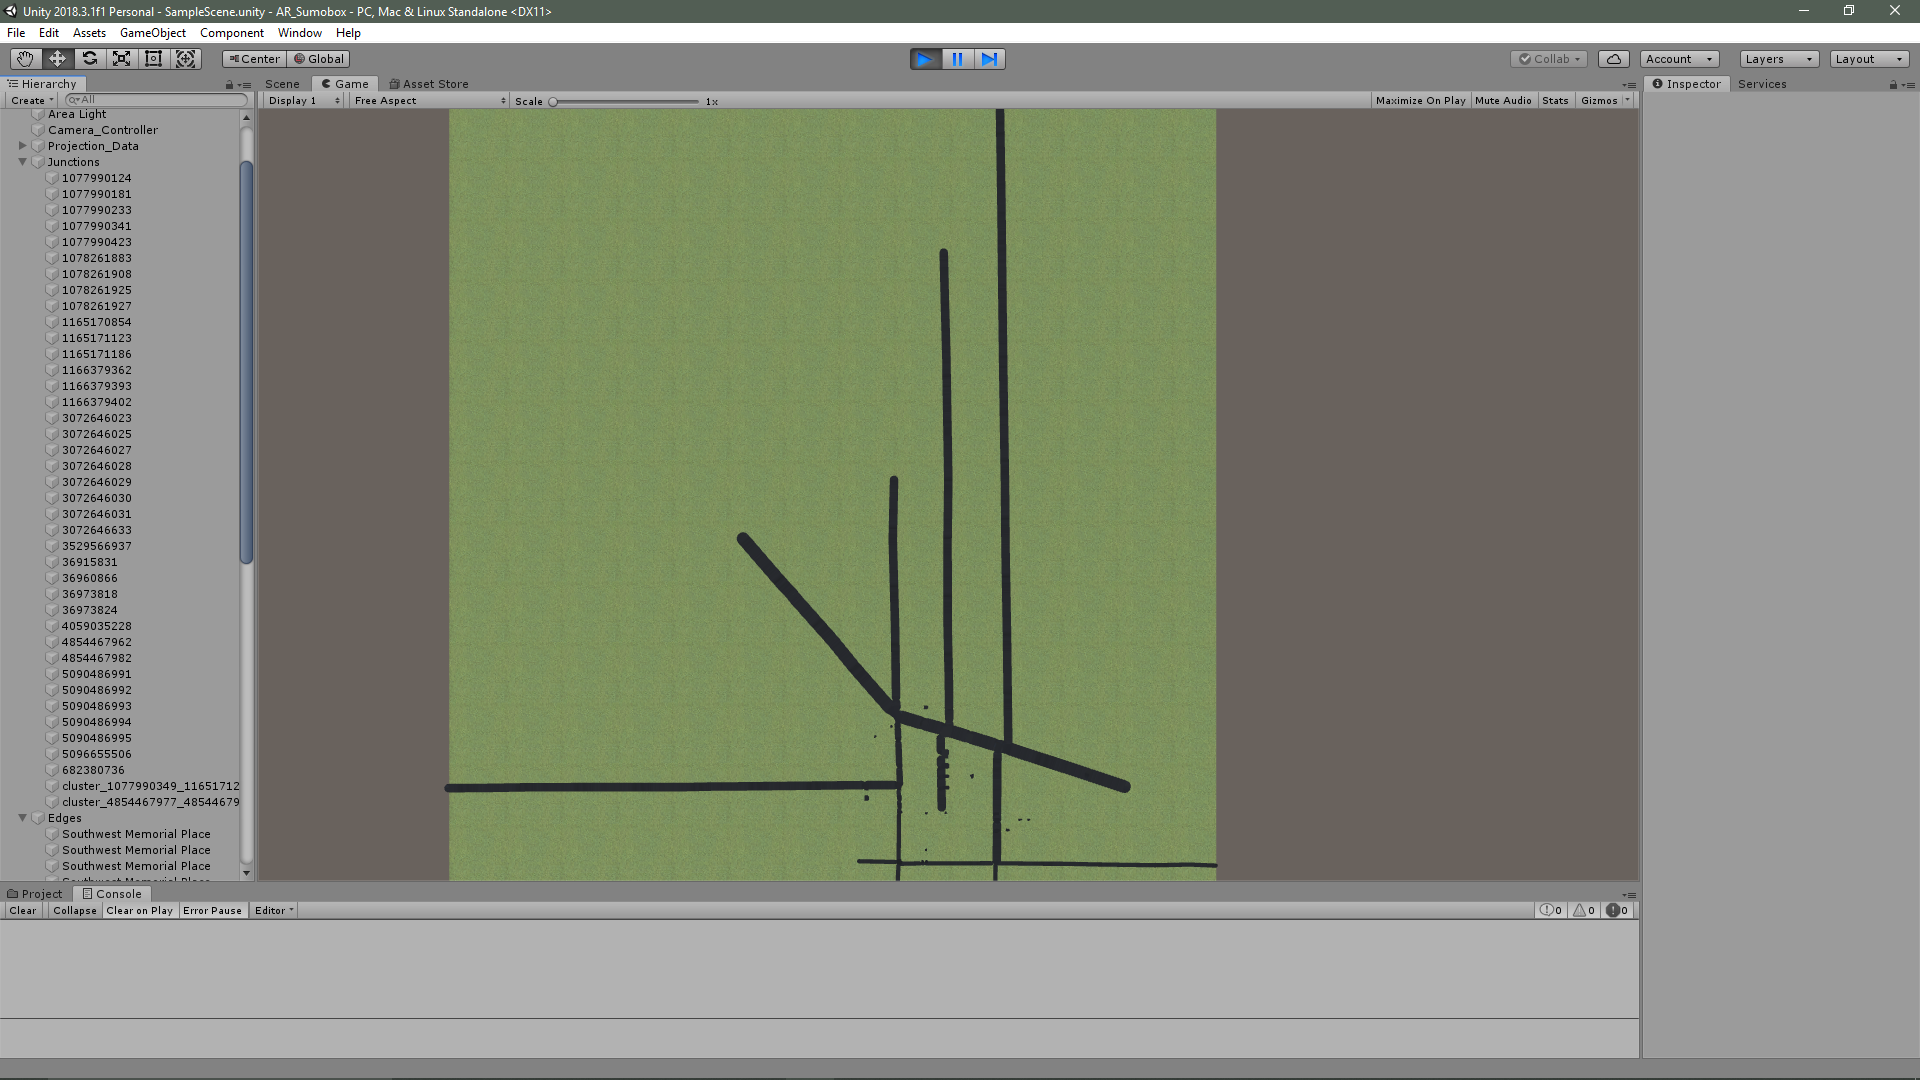
\includegraphics[width=\textwidth]{CloseupJunctions_13}
    \caption{Another view of the network with the list of its "Junctions" expanded for reference.}
    \label{fig:my_label}
\end{figure}
\vspace{3pt}
\begin{figure}[h!]
    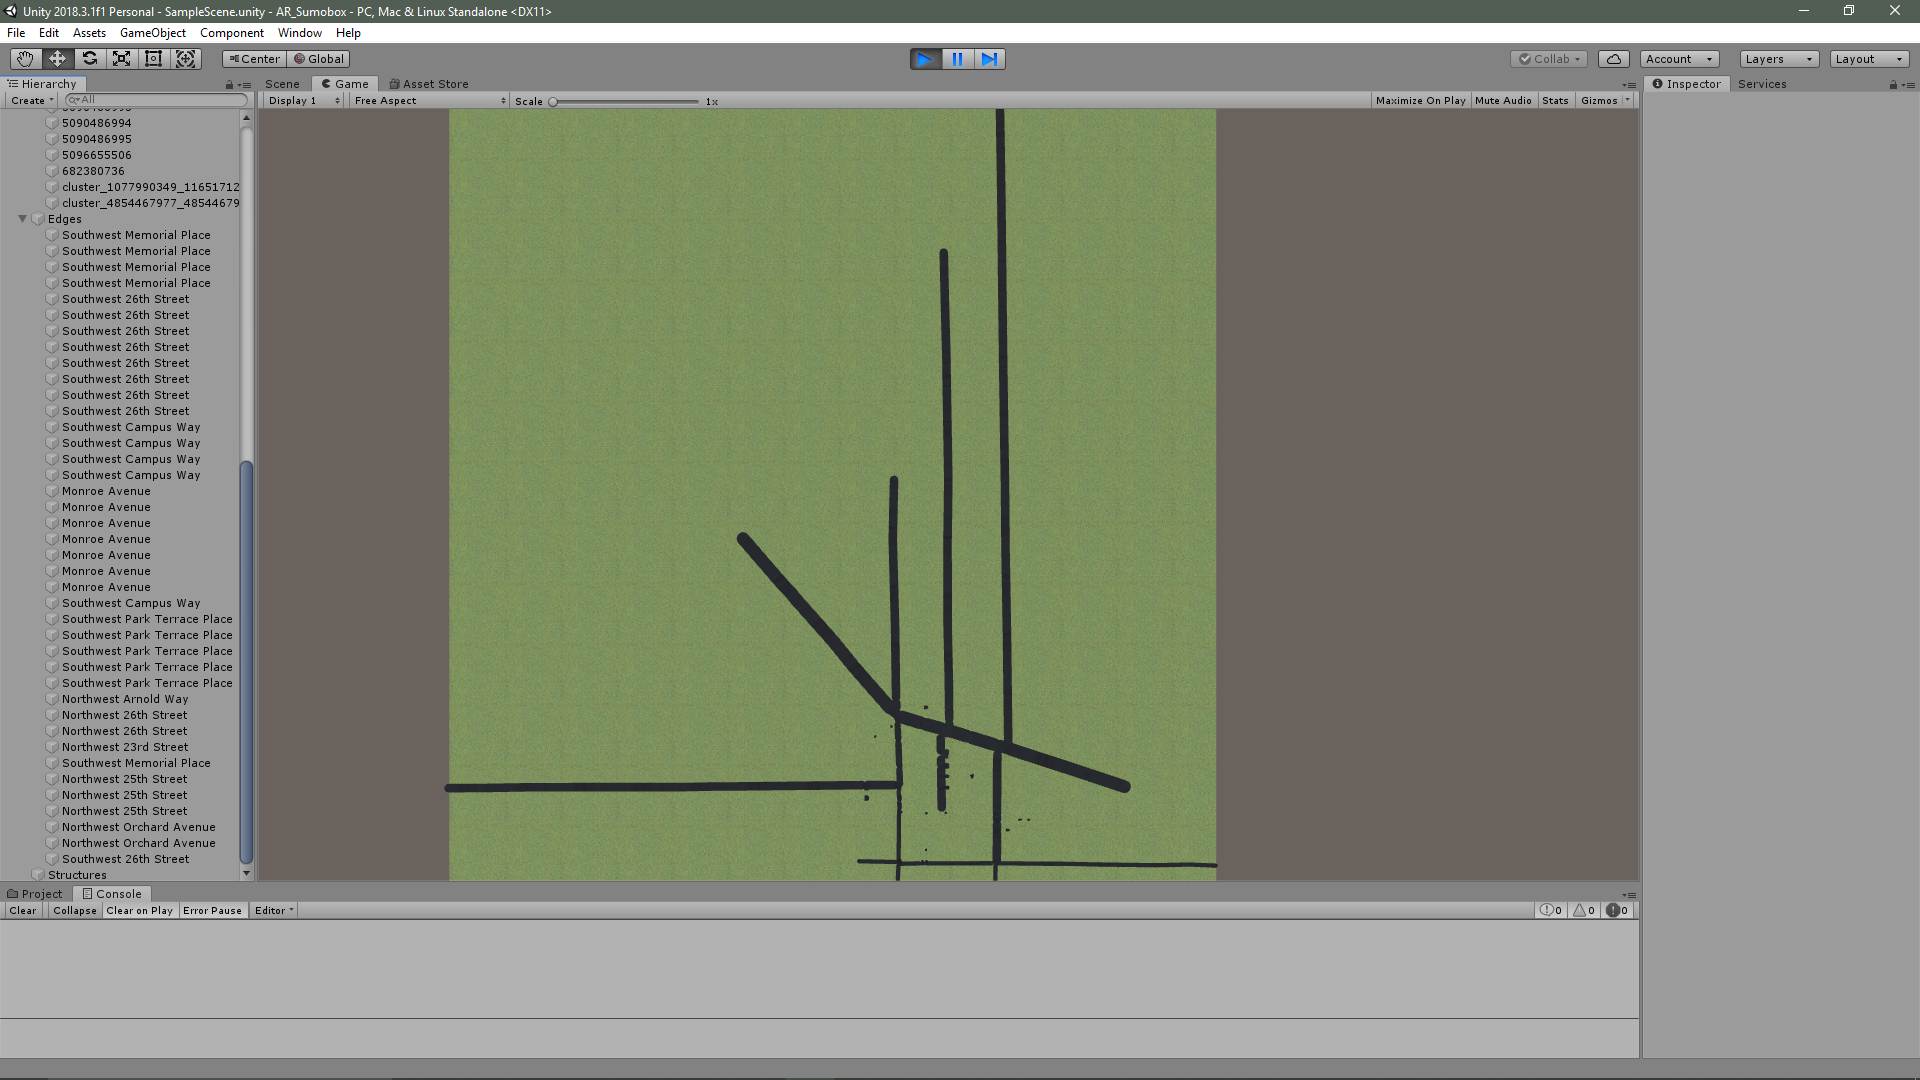
\includegraphics[width=\textwidth]{CloseupEdges_14}
    \caption{Another view of the network with the list of its "Edges" expanded for reference.}
    \label{fig:my_label}
\end{figure}
    
% Code Samples
% SumoCreator.cs Class file
\newpage
\section{Traffic Simulation Network Creation Classes}
    \begin{lstlisting}[language=c, style=mystyle, caption=SumoCreator.cs]
        // SumoCreator class is used for creating Open Street Map networks with SUMO's
        // OSM Web Wizard and reading SUMO generated files that describe a networks logic 
        // and layout. 
        public class SumoCreator : MonoBehaviour
        {
            // ProjectionData Parent GameObject and script.
            private GameObject Projection_Data_GO;
            
            // Junctions Parent GameObject and script.
            private GameObject Junctions_GO;
            
            // Edges Parent GameObject and script.
            private GameObject Edges_GO;
            
            // Structures Parent GameObject and script. 
            private GameObject Structures_GO;
            
            // Starts off the SumoCreator
            private void Start()
            {
                Projection_Data_GO = GameObject.Find("Projection_Data");
                Junctions_GO = GameObject.Find("Junctions");
                Edges_GO = GameObject.Find("Edges");
                Structures_GO = GameObject.Find("Structures");
            }
        
            
            // Builds the network pieces by reading a Sumo network file.
            // Reads through a network and saves all the network data to the handling class.
            // There are classes for ProjectionData, Edge, and Junction.
            // After all data is read in each class builds its own shapes. 
            private void BuildNetwork(string file)
            {
                ...
            }
            
            // Builds the structures of the given file
            private void BuildStructures(string file)
            {
                ...
            }
        
            // Open Up OSMWebWizard and let the user build a real network.
            // The user will save the new network to a zipfile when done.
            // The processes remain open so the user can build multiple network at once.
            public void GenerateOsmNetwork()
            {
                ...
            }
        
            // Go through all network description files and build the network into Unity.
            // Most files will be passed over at this point but there are some handles left 
            // in case we decide we need access to them later.
            public void LoadNetwork()
            {
                ...
            }
        }
    \end{lstlisting}

%SECTION APPENDICES
\newpage
\appendices

%SECTION REFS
\newpage
\bibliographystyle{IEEEtran}
\bibliography{references}
        
\end{document}
